\documentclass{report}
\usepackage{graphicx, tikz-cd, float, titlepic, booktabs} % Required for inserting images
\usepackage{pgfplots}
\pgfplotsset{compat=1.15}
\usepackage{mathrsfs}
\usetikzlibrary{arrows}
\usepackage{amsmath, amssymb, amsthm, amsfonts, siunitx, physics, gensymb}
\AtBeginDocument{\RenewCommandCopy\qty\SI}
\usepackage[version=4]{mhchem}
\usepackage[most,many,breakable]{tcolorbox}
\usepackage{xcolor, fancyhdr, varwidth}
\usepackage[Glenn]{fncychap}
%Options: Sonny, Lenny, Glenn, Conny, Rejne, Bjarne, Bjornstrup
\usepackage{hyperref, cleveref}
\usepackage{icomma, enumitem} %comma as decimal and continue enumerate with [resume]
\usepackage[danish]{babel}
%%%%%%%%%%%%%%%%%%%%%%%%%%%%%%
% SELF MADE COLORS
%%%%%%%%%%%%%%%%%%%%%%%%%%%%%%
\definecolor{myg}{RGB}{56, 140, 70}
\definecolor{myb}{RGB}{45, 111, 177}
\definecolor{myr}{RGB}{199, 68, 64}
\definecolor{mytheorembg}{HTML}{F2F2F9}
\definecolor{mytheoremfr}{HTML}{00007B}
\definecolor{mylenmabg}{HTML}{FFFAF8}
\definecolor{mylenmafr}{HTML}{983b0f}
\definecolor{mypropbg}{HTML}{f2fbfc}
\definecolor{mypropfr}{HTML}{191971}
\definecolor{myexamplebg}{HTML}{F2FBF8}
\definecolor{myexamplefr}{HTML}{88D6D1}
\definecolor{myexampleti}{HTML}{2A7F7F}
\definecolor{mydefinitbg}{HTML}{E5E5FF}
\definecolor{mydefinitfr}{HTML}{3F3FA3}
\definecolor{notesgreen}{RGB}{0,162,0}
\definecolor{myp}{RGB}{197, 92, 212}
\definecolor{mygr}{HTML}{2C3338}
\definecolor{myred}{RGB}{127,0,0}
\definecolor{myyellow}{RGB}{169,121,69}
\definecolor{myexercisebg}{HTML}{F2FBF8}
\definecolor{myexercisefg}{HTML}{88D6D1}
%%%%%%%%%%%%%%%%%%%%%%%%%%%%%%%%%%%%%%%%%%%%%%%%%%%%%%%%%%%%%%%%%%%%%%
% Box environments for theorems and problems
%%%%%%%%%%%%%%%%%%%%%%%%%%%%%%%%%%%%%%%%%%%%%%%%%%%%%%%%%%%%%%%%%%%%%
\setlength{\parindent}{1cm}
%================================
% Question BOX
%================================
\makeatletter
\newtcbtheorem{question}{Opgave}{enhanced,
	breakable,
	colback=white,
	colframe=myb!80!black,
	attach boxed title to top left={yshift*=-\tcboxedtitleheight},
	fonttitle=\bfseries,
	title={#2},
	boxed title size=title,
	boxed title style={%
			sharp corners,
			rounded corners=northwest,
			colback=tcbcolframe,
			boxrule=0pt,
		},
	underlay boxed title={%
			\path[fill=tcbcolframe] (title.south west)--(title.south east)
			to[out=0, in=180] ([xshift=5mm]title.east)--
			(title.center-|frame.east)
			[rounded corners=\kvtcb@arc] |-
			(frame.north) -| cycle;
		},
	#1
}{def}
\makeatother
%================================
% DEFINITION BOX
%================================

\newtcbtheorem[]{Definition}{Definition}{enhanced,
	before skip=2mm,after skip=2mm, colback=red!5,colframe=red!80!black,boxrule=0.5mm,
	attach boxed title to top left={xshift=1cm,yshift*=1mm-\tcboxedtitleheight}, varwidth boxed title*=-3cm,
	boxed title style={frame code={
					\path[fill=tcbcolback]
					([yshift=-1mm,xshift=-1mm]frame.north west)
					arc[start angle=0,end angle=180,radius=1mm]
					([yshift=-1mm,xshift=1mm]frame.north east)
					arc[start angle=180,end angle=0,radius=1mm];
					\path[left color=tcbcolback!60!black,right color=tcbcolback!60!black,
						middle color=tcbcolback!80!black]
					([xshift=-2mm]frame.north west) -- ([xshift=2mm]frame.north east)
					[rounded corners=1mm]-- ([xshift=1mm,yshift=-1mm]frame.north east)
					-- (frame.south east) -- (frame.south west)
					-- ([xshift=-1mm,yshift=-1mm]frame.north west)
					[sharp corners]-- cycle;
				},interior engine=empty,
		},
	fonttitle=\bfseries,
	title={#2},#1}{def}
\newtcbtheorem[]{definition}{Definition}{enhanced,
	before skip=2mm,after skip=2mm, colback=red!5,colframe=red!80!black,boxrule=0.5mm,
	attach boxed title to top left={xshift=1cm,yshift*=1mm-\tcboxedtitleheight}, varwidth boxed title*=-3cm,
	boxed title style={frame code={
					\path[fill=tcbcolback]
					([yshift=-1mm,xshift=-1mm]frame.north west)
					arc[start angle=0,end angle=180,radius=1mm]
					([yshift=-1mm,xshift=1mm]frame.north east)
					arc[start angle=180,end angle=0,radius=1mm];
					\path[left color=tcbcolback!60!black,right color=tcbcolback!60!black,
						middle color=tcbcolback!80!black]
					([xshift=-2mm]frame.north west) -- ([xshift=2mm]frame.north east)
					[rounded corners=1mm]-- ([xshift=1mm,yshift=-1mm]frame.north east)
					-- (frame.south east) -- (frame.south west)
					-- ([xshift=-1mm,yshift=-1mm]frame.north west)
					[sharp corners]-- cycle;
				},interior engine=empty,
		},
	fonttitle=\bfseries,
	title={#2},#1}{def}

\newtcbtheorem{theo}%
    {Theorem}{}{theorem}
\newtcolorbox{prob}[1]{colback=red!5!white,colframe=red!50!black,fonttitle=\bfseries,title={#1}}
%================================
% NOTE BOX
%================================

\usetikzlibrary{arrows,calc,shadows.blur}
\tcbuselibrary{skins}
\newtcolorbox{note}[1][]{%
	enhanced jigsaw,
	colback=gray!20!white,%
	colframe=gray!80!black,
	size=small,
	boxrule=1pt,
	title=\textbf{Note:},
	halign title=flush center,
	coltitle=black,
	breakable,
	drop shadow=black!50!white,
	attach boxed title to top left={xshift=1cm,yshift=-\tcboxedtitleheight/2,yshifttext=-\tcboxedtitleheight/2},
	minipage boxed title=1.5cm,
	boxed title style={%
			colback=white,
			size=fbox,
			boxrule=1pt,
			boxsep=2pt,
			underlay={%
					\coordinate (dotA) at ($(interior.west) + (-0.5pt,0)$);
					\coordinate (dotB) at ($(interior.east) + (0.5pt,0)$);
					\begin{scope}
						\clip (interior.north west) rectangle ([xshift=3ex]interior.east);
						\filldraw [white, blur shadow={shadow opacity=60, shadow yshift=-.75ex}, rounded corners=2pt] (interior.north west) rectangle (interior.south east);
					\end{scope}
					\begin{scope}[gray!80!black]
						\fill (dotA) circle (2pt);
						\fill (dotB) circle (2pt);
					\end{scope}
				},
		},
	#1,
}
%================================
% EXAMPLE BOX
%================================
\newtcbtheorem[number within=section]{Example}{Example}
{%
	colback = myexamplebg
	,breakable
	,colframe = myexamplefr
	,coltitle = myexampleti
	,boxrule = 1pt
	,sharp corners
	,detach title
	,before upper=\tcbtitle\par\smallskip
	,fonttitle = \bfseries
	,description font = \mdseries
	,separator sign none
	,description delimiters parenthesis
}
{ex}
%================================
% THEOREM BOX
%================================

\tcbuselibrary{theorems,skins,hooks}
\newtcbtheorem[number within=section]{Theorem}{Theorem}
{%
	enhanced,
	breakable,
	colback = mytheorembg,
	frame hidden,
	boxrule = 0sp,
	borderline west = {2pt}{0pt}{mytheoremfr},
	sharp corners,
	detach title,
	before upper = \tcbtitle\par\smallskip,
	coltitle = mytheoremfr,
	fonttitle = \bfseries\sffamily,
	description font = \mdseries,
	separator sign none,
	segmentation style={solid, mytheoremfr},
}
{th}

%%%%%%%%%%%%%%%%%%%%%%%%%%%%%%%%%%%%%%%%%%%%%%%%%%%%%%%%%%%%%%%%%
% SELF MADE COMMANDS
%%%%%%%%%%%%%%%%%%%%%%%%%%%%%%
\newcommand{\sol}{\setlength{\parindent}{0cm}\textbf{\textit{Løsning:}}\setlength{\parindent}{1cm}}
%%%%%%%%%%%%%%%%%%%%%%%%%%%%%%%%%
\usepackage[tmargin=2cm,rmargin=1in,lmargin=1in,margin=0.85in,bmargin=2cm,footskip=.2in]{geometry}\pagestyle{fancy}
\lhead{Virum Gymnasium}
\rhead{Skriftlig årsprøve}

\title{Skriftlig årsprøve\\
{\Large \textbf{Kemi A}}}
\author{Kevin Zhou}
\date{\today}

\begin{document}
\maketitle
\begin{note}
  Ved besvarelsen er anvendt Databogen 11. udgave 2007
\end{note}
\section*{Opgave 1}
\sol \\
\textbf{a.}
Vi ser på titrerkurven, at ækvivalenspunktet ligger omkring $pH=9,00$.
Vi vil altså gerne bruge en indikator, hvis omslagsområde er deromkring. 
Phenolphthalein ville da være  en egnet indikator til en kolorimetrisk titrering af syren med natriumhydroxidopløsningen, da dens omslagsområde ligger i $pH \in [8,2;10,0]$.\\[1ex]
\textbf{b.}
Det tilsatte volumen natriumhydroxidopløsning ved ækvivalenspunktet aflæses til at være $25,25 \;\unit{mL} $.
Vi beregner nu stofmængden af tilsat natriumhydroxid.
\begin{equation*}
\begin{split}
  n(\ce{NaOH} )&= V \cdot c(\ce{NaOH} )\\ 
  &= 25,25 \;\unit{mL} \cdot 0,0986 \;\unit{\textsc{m}} \\ 
  &=2,48965 \;\unit{mmol} 
\end{split}
\end{equation*}
Ved titrering af syre med base er reaktionsforholdet mellem disse 1:1.
\begin{equation*}
\begin{split}
  n(\text{syre})&=n(\ce{NaOH} )\\ 
  &\approx 2,49 \;\unit{mmol} 
\end{split}
\end{equation*}
Da vi både kender massen og stofmængden af carboxylsyren kan vi udregne dens molare masse.
\begin{equation*}
\begin{split}
  M(\text{syre} )&=\frac{m(\text{syre} )}{n(\text{syre} )}\\ 
  &=\frac{0,254 \;\unit{g} }{2,48965 \cdot 10^{-3} \;\unit{mol} }\\ 
  &\approx 102 \;\unit{g/mol} 
\end{split}
\end{equation*}
Altså er stofmængden af den monohydrone carboxylsyre $2,49 \;\unit{mmol} $ og dens molare masse $102 \;\unit{g/mol} $.\\[1ex]
\textbf{c.}
Nedenfor i \cref{fig:carbox} ses 2 forskellige strukturformler for carboxylsyrer med strukturformlen \ce{C5H10O2}.
\begin{figure}[H]
\begin{center}
  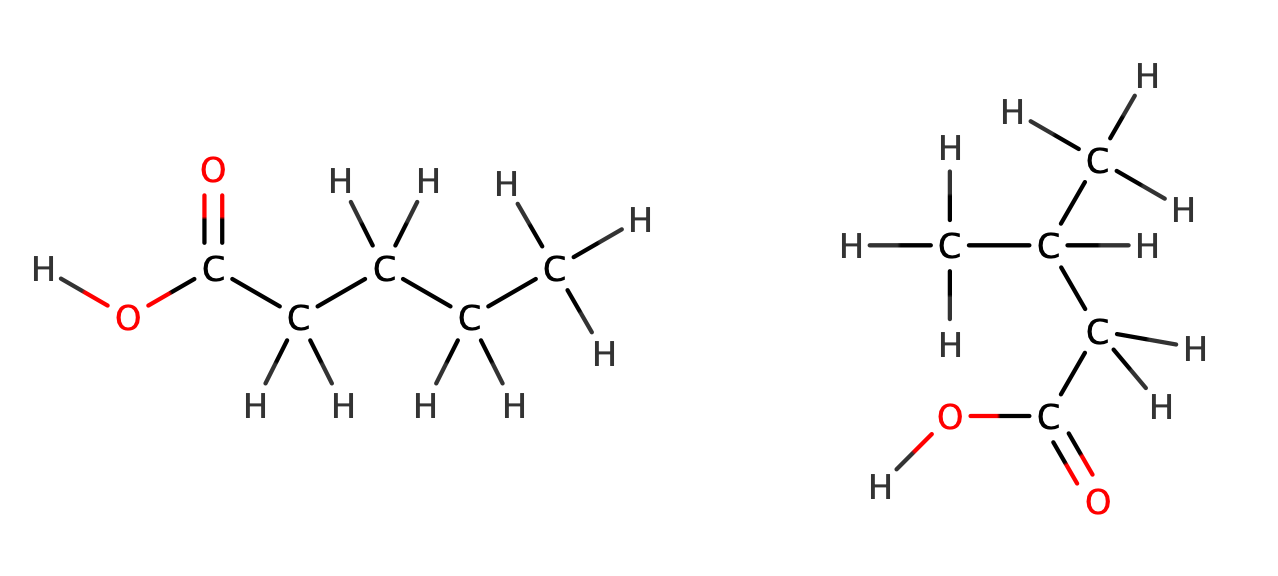
\includegraphics[width=\textwidth]{carbox.png}
\end{center}
\caption{To forskellige strukturformler tegnet i MarvinSketch}
\label{fig:carbox}
\end{figure}

\section*{Opgave 2}
\sol \\
\textbf{a.}
Både lawson og stof A kan addere dibrom. 
Siden det kun er reagensglas 2, der er farvet, så må det være stoffet B, der er anbragt i glas 2.
Carbonylforbindelser bliver påvist af 2,4-dinitrophenylhydrazin, idet der dannes tungtopløselige hydrazoner, der er gule/orange.
Da lawson og B begge er ketoner, hvor A ikke indeholder carbonylgruppen, samt at der dannes bundfald i glas 2 og glas 3, så må lawson være anbragt i glas 3 og A må være anbragt i glas 1. \\[1ex]
\textbf{b.}
Man bør måle absorbanserne for opløsningerne af lawson ved $452 \;\unit{nm} $, hvor der er maksimal absorbans, da en lille ændring i $c(\text{lawson} )$ kun ville give en relativt lille ændring i absorbansen. 
Altså ville usikkerheder have den mindste betydning der.

Der er maksimal absorbans ved $452 \;\unit{nm} $, hvilket er bølgelængden på farven blå.
Da stoffets farve vil være komplementærfarven af den farve, den absorberer, så vil en opløsning af lawson have farven orange.\\[1ex]
\textbf{c.}
Standardkurven for lawson ses tegnet i \cref{fig:absorbans}.
\begin{figure}[H]
\begin{center}
  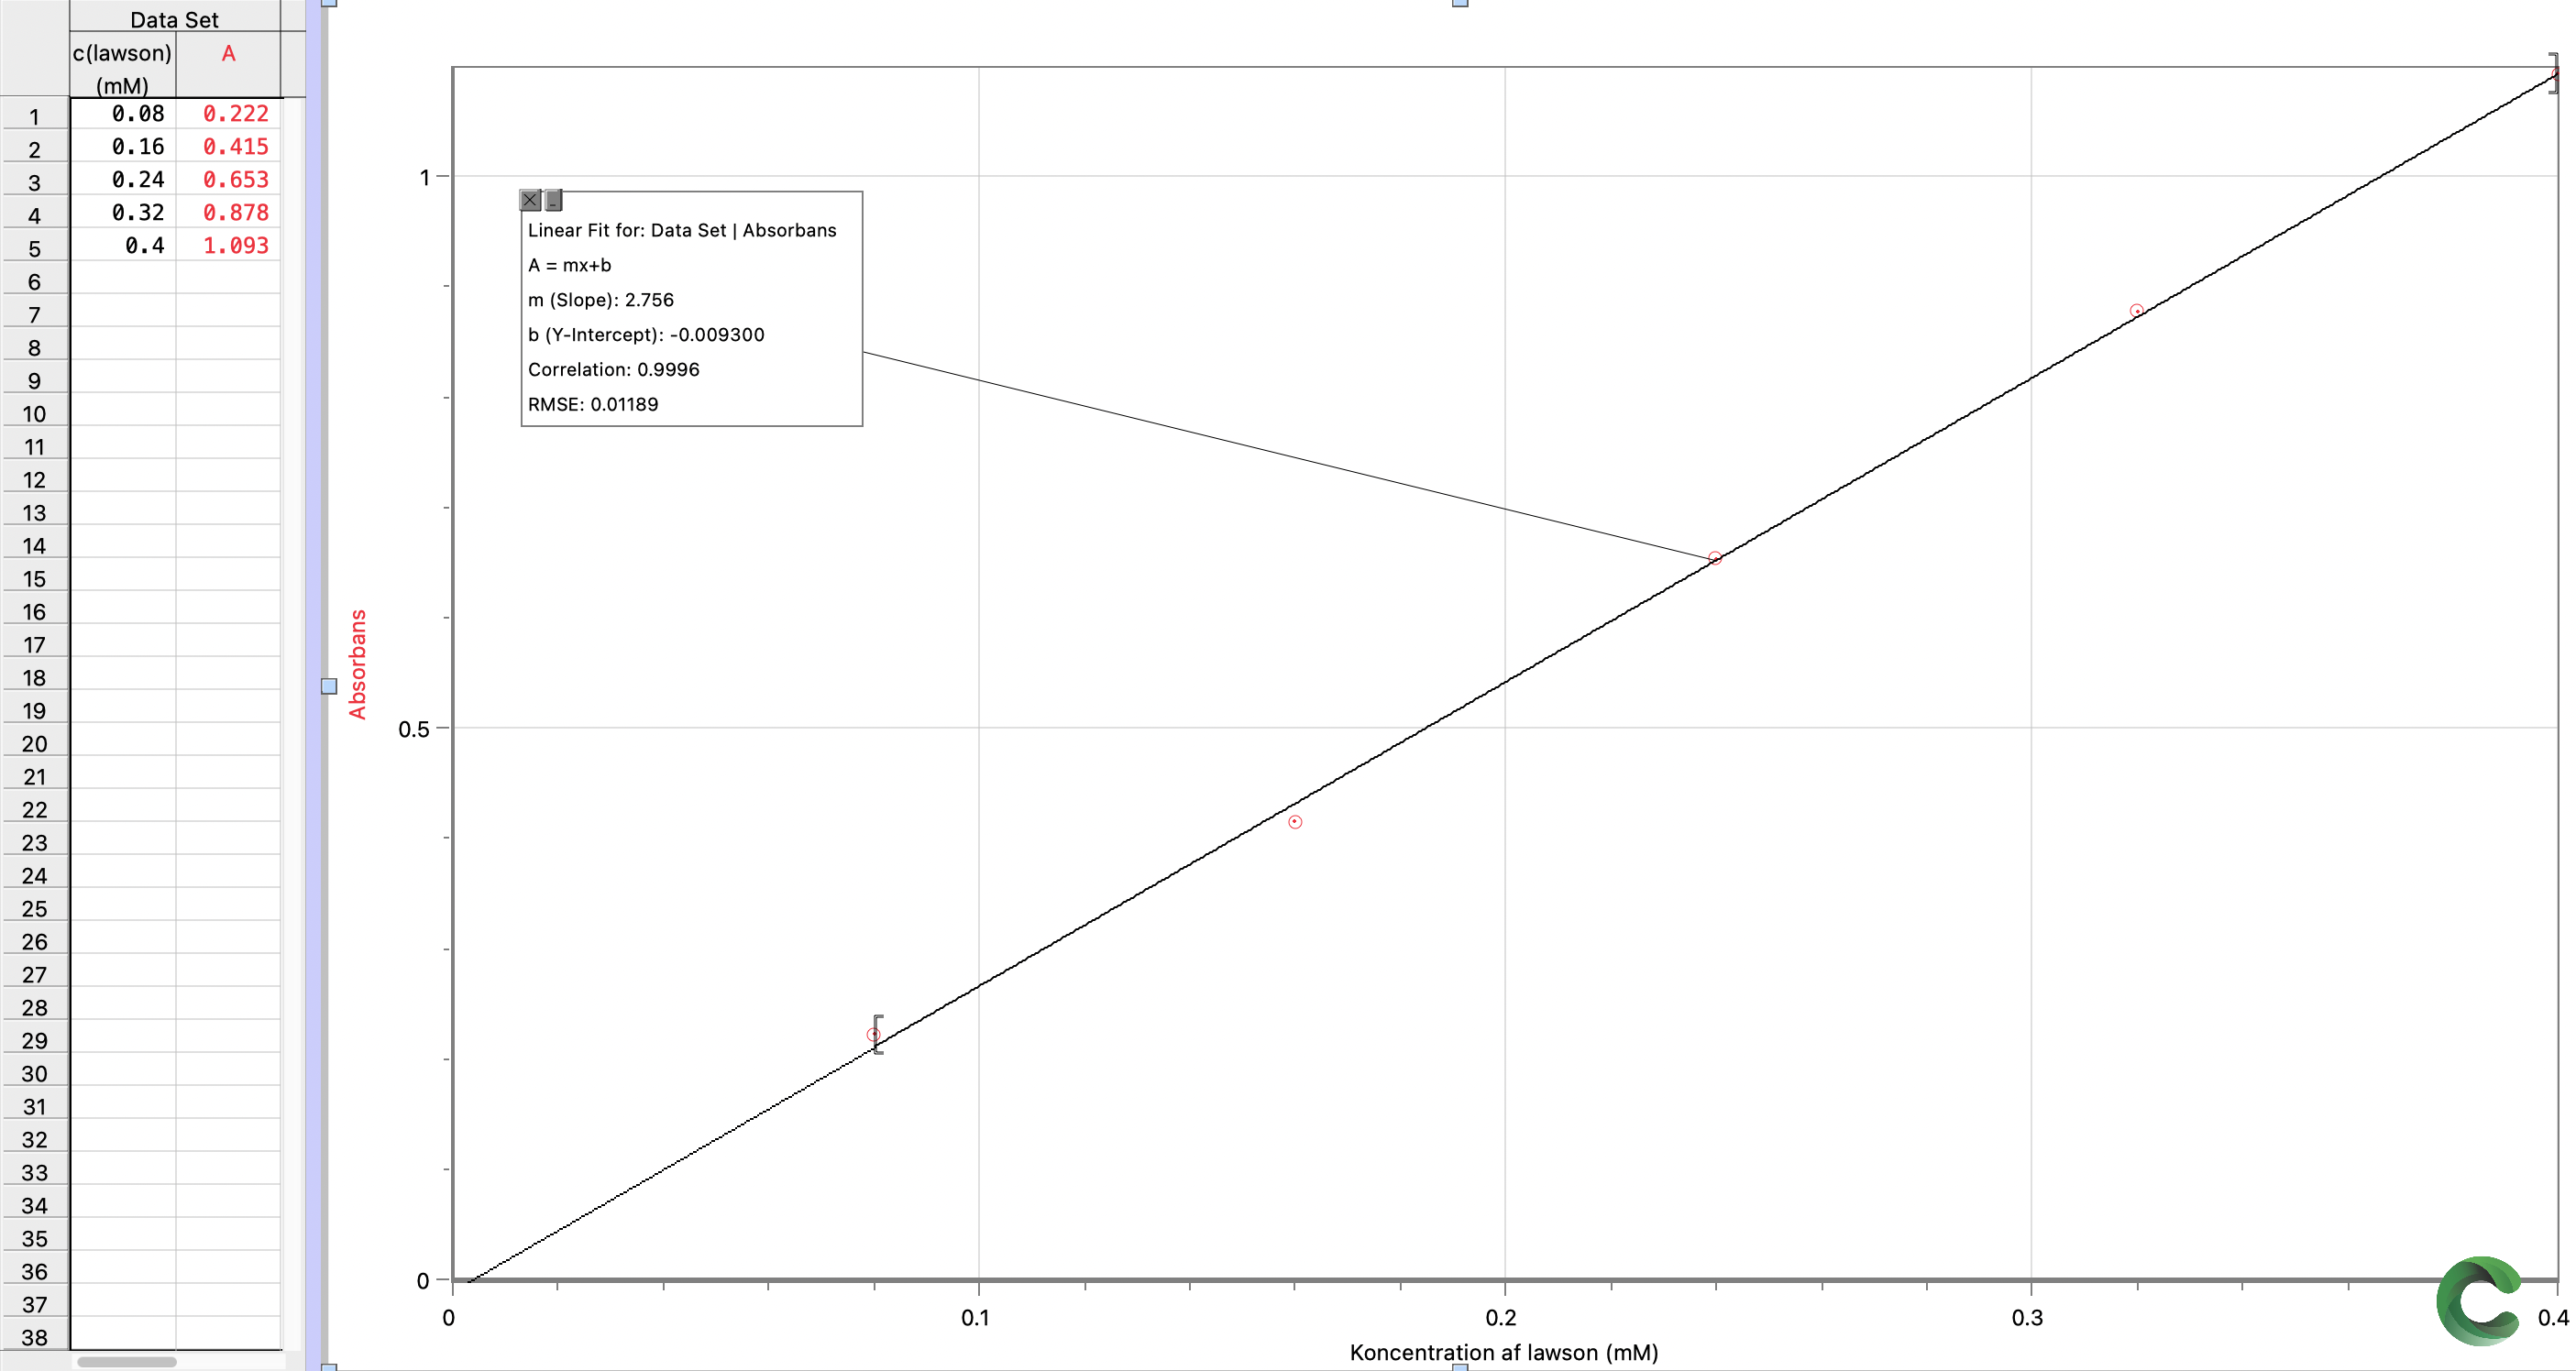
\includegraphics[width=\textwidth]{absorbans.png}
\end{center}
\caption{Standardkurven for lawson tegnet i LoggerPro}
\label{fig:absorbans}
\end{figure}
Siden målepunkterne ligger på en ret linje, der tilnærmelsesvist går gennem (0,0), tyder det på, at absorbansen er proportional med koncentrationen af lawson.
Altså følger absorbansen Lambert-Beers lov for lawson i standardopløsningerne.\\[1ex]
\textbf{d.}
Fra \textbf{c.} har vi, at 
\begin{equation*}
\begin{split}
  A=2,756 \cdot \frac{c(lawson)}{\;\unit{m \textsc{m}}} - 0,0093 \iff c(lawson)= \frac{A+ 0,0093}{2,756} \;\unit{m \textsc{m}} 
\end{split}
\end{equation*}
Vi kan nu regne stofmængdekoncentrationen af lawson ud i $50 \;\unit{mL} $ målekolben. 
\begin{equation*}
\begin{split}
  c(lawson)&= \frac{A+ 0,0093}{2,756} \;\unit{m \textsc{m}} \\ 
  &= \frac{0,262 + 0,0093}{2,756} \;\unit{m \textsc{m}} \\ 
  &\approx 0,0984 \;\unit{m \textsc{m} } 
\end{split}
\end{equation*}
Vi bestemmer nu indholdet af lawson i hennapulveret.
\begin{equation*}
\begin{split}
  \frac{m(lawson)}{m(henna)}&= \frac{c(lawson) \cdot V}{m(henna)}\\ 
  &=\frac{c(lawson) \cdot 5,0 \cdot 10^{-2} \;\unit{L} }{0,121 \;\unit{g} }\\ 
  &\approx 4,1 \cdot 10^{-2} \;\unit{mg/g} 
\end{split}
\end{equation*}
Altså har vi fået stofmængdekoncentrationen af lawson i målekolben til at være $0,0984 \;\unit{m \textsc{m}} $ og indholdet af lawson i hennapulveret til at være $4,1 \cdot 10^{-2} \;\unit{mg/g} $.

\section*{Opgave 3}
\sol \\
\textbf{a.}
Syregruppen er den højst prioriterede funktionelle gruppe, som glycolsyren indholder. 
Derfor får det systematiske navn suffikset -syre, og vi nummererer \ce{C}-atomerne fra højre side (hvor syregruppen sidder).
Da den længste kæde af \ce{C}-atomer er 2, så skal ethan være i navnet.
Derudover sidder en hydroxygruppe på 2. \ce{C}-atom. 
Det angives med præfikset 2-hydroxy.
Altså må det systematiske navn være 2-hydroxyethansyre.\\[1ex]
\textbf{b.}
Den formelle stofmængdekoncentration af mælkesyre i opløsning A må være 
\begin{equation*}
\begin{split}
  c(\text{mælkesyre} )&= \frac{n(\text{mælkesyre} )}{V}\\ 
  &=\frac{\frac{m(\text{mælkesyre} )}{M(\text{mælkesyre} )}}{V}\\ 
  &=\frac{\frac{3,00 \;\unit{g} }{90,08 \;\unit{g/mol} }}{0,100 \;\unit{L} }\\ 
  &\approx 0,333 \;\unit{\textsc{m}} 
\end{split}
\end{equation*}
Hvilket var det, der skulle vises.\\[1ex]
\textbf{c.}
Vi regner $K_s$ for mælkesyre ud. 
\begin{equation*}
\begin{split}
  K_s&=10^{-pK_s} \;\unit{\textsc{m}} \\ 
  &=10^{-3,86} \;\unit{\textsc{m}} \\ 
  &=1,38038 \cdot 10^{-4} \;\unit{\textsc{m}} 
\end{split}
\end{equation*}
Siden mælkesyre er en middelstærk syre, hvor der gælder, at
\[
K_s=\frac{[\ce{H3O+} ]^2}{c_s - [\ce{ H3O+}]}
\] 
så har vi, at 
\begin{equation*}
\begin{split}
  [\ce{H3O+}]&=\frac{-K_s^2 + \sqrt{K_s^2- 4 \cdot 1 \cdot (-c(\text{mælkesyre} ) \cdot K_s)} }{2 \cdot 1}\\ 
  &=\frac{-(1,38038 \cdot 10^{-4} \;\unit{\textsc{m}})^2 + \sqrt{(1,38038 \cdot 10^{-4} \;\unit{\textsc{m}})^2- 4\cdot (-0,333 \;\unit{\textsc{m}}  \cdot 1,38038 \cdot 10^{-4} \;\unit{\textsc{m}})} }{2}\\ 
  &=0,006780223 \;\unit{\textsc{m}} 
\end{split}
\end{equation*}
Vi regner nu pH ud.
\begin{equation*}
\begin{split}
  pH&=-\log \left(\frac{[\ce{H3O+} ]}{\;\unit{\textsc{m}} }\right) \\ 
  &=-\log \left(\frac{0,006780223 \;\unit{\textsc{m}} }{\;\unit{\textsc{m}} }\right) \\ 
  &\approx 2,17
\end{split}
\end{equation*}
Altså har vi regnet at $K_s=1,38 \cdot 10^{-4} \;\unit{\textsc{m}} $ og pH i opløsning A til at være $2,17$. 

\section*{Opgave 4}
\sol \\
\textbf{a.}
En grim afstemning af redoxreaktionen ses i \cref{fig:redox}.
\begin{figure}[H]
\begin{center}
  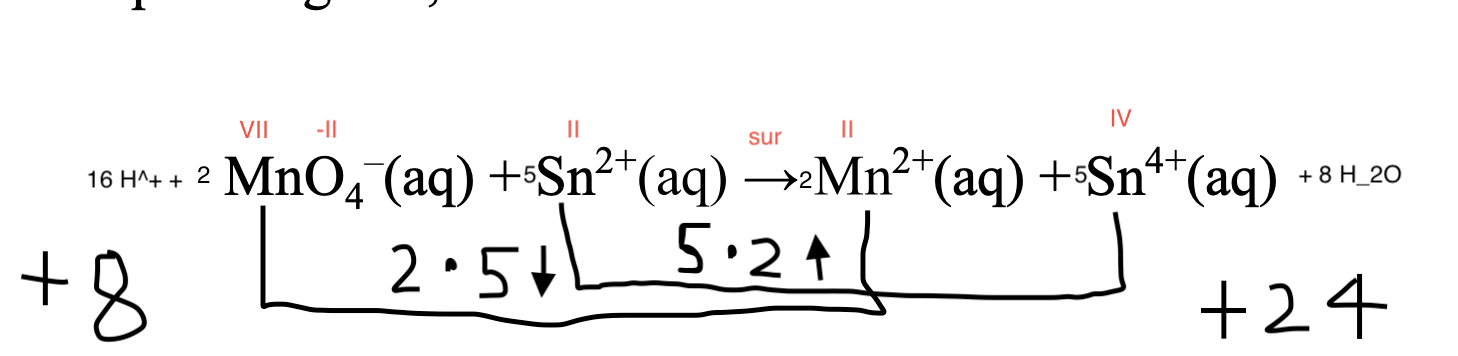
\includegraphics[width=\textwidth]{redox.png}
\end{center}
\caption{Redoxreaktionen afstemt med tegneværktøjer}
\label{fig:redox}
\end{figure}
Det afstemte reaktionsskema ville altså se således ud: 
\[
\ce{2MnO4-(aq) + 5 Sn^2+(aq) + 16 H+(aq) -> 2 Mn^2+(aq) + 5 Sn^4+(aq) + 8 H2O(l)} 
\] 

\section*{Opgave 5}
\sol \\
\textbf{a.}
Da opløsningsmidlet indgår i reaktionsbrøken med stofmængdebrøken, er ligevægtsloven for ligevægten 
\[
\frac{[\ce{Cr_2O7^2-} ]}{[\ce{H3O+} ]^2 \cdot [\ce{CrO4^2-} ]^2}=K
\] 
\textbf{b.}
Ved tilsætning af koncentreret saltsyre bliver $[\ce{H3O+} ]$ større. 
Dette gør reaktionsbrøken mindre end $K$, og en forskydning mod højre følger.
Den større koncentraiton af dichromat gør opløsningen mere orange: 
\[
\frac{[\ce{Cr_2O7^2-} ]}{[\ce{H3O+} ]^2 \cdot [\ce{CrO4^2-} ]^2}<K \quad \ce{->} 
\] 

\section*{Opgave 6}
\sol \\
\textbf{a.}
I \cref{fig:leucin} ses, at der er ét assymetrisk \ce{C}-atom i leucin.
\begin{figure}[H]
\begin{center}
  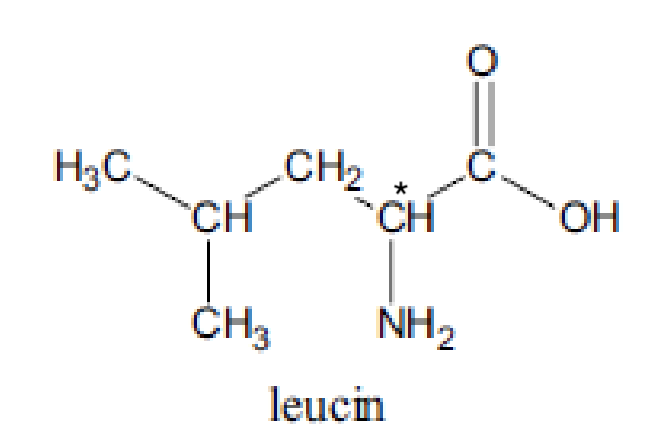
\includegraphics[scale=1]{leucin.png}
\end{center}
\caption{Strukturformel for leucin, hvor det assymetriske \ce{C}-atom er markeret}
\label{fig:leucin}
\end{figure}
Da leucin indeholder ét assymetrisk \ce{C}-atom, så må der findes 2 spejlbilledisomere former for det.\\[1ex]
\textbf{b.}
Reaktionstypen for reaktion I er en oxidationsreaktion.
Der er tale om en oxidation, da vi ser et aldehyd blive oxideret til en carboxylsyre.
Reaktionstypen for reaktion V er en kondensationsreaktion, hvor en sammenbinding sker af to organiske molekyler under fraspaltning af et vandmolekyle sker.
Der fremkommer da en ether.
Reaktanten i \cref{fig:reaktant} skal reagere med stof C for at fremstille stof F.
Dette er tilfældet, da etheren i stof F fremkommer, når de to stoffer kondenserer.
\begin{figure}[H]
\begin{center}
  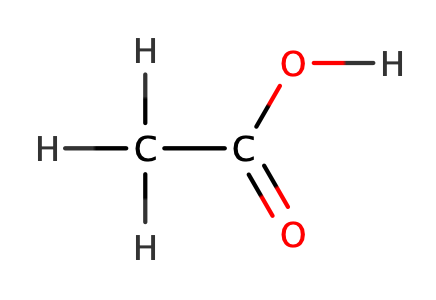
\includegraphics[scale=1]{reaktant.png}
\end{center}
\caption{Strukturformlen for ethansyre}
\label{fig:reaktant}
\end{figure}
\textbf{c.} 
Stof E er en ester. 
Estergruppen kan ses markeret i \cref{fig:E}.
\begin{figure}[H]
\begin{center}
  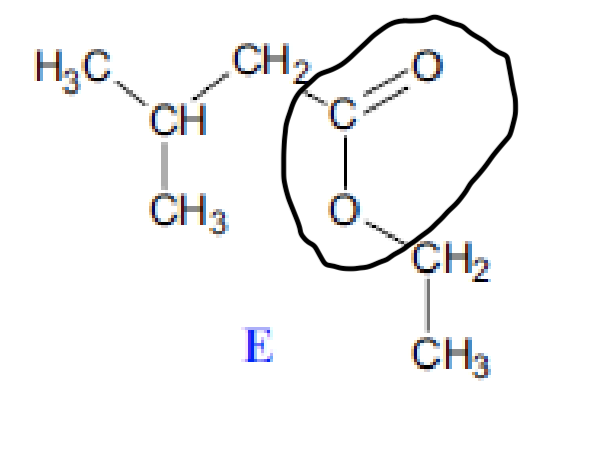
\includegraphics[scale=1]{E.png}
\end{center}
\caption{Estergruppen markeret i strukturformlen for E}
\label{fig:E}
\end{figure}
Vi ser, at stof E indholder 1 hydrofil gruppe (carbonylgruppen), mens den indholder 6 \ce{C}-atomer med hydrofobe grupper.
Siden tommelfingerreglen er, at 4 carbonatomer med hydrofobe grupper ophæver virkningen af en hydrofil gruppe, så er stof E så godt som uopløselig i vand.

\end{document}
